\section{Độ dài của cung tròn, Diện tích hình quạt tròn và hình vành khuyên.} % Tên bài
\subsection{Độ dài cung tròn.}
\subsubsection{Kiến thức trọng tâm.}
\begin{tomtat}
	\begin{boxdn}
		\begin{itemize}
			\item Chu vi của một đường tròn tâm $O$, bán kính $R$ là
			\begin{center}
				$C=2\pi R=d\pi$ ($d$ là đường kính).
			\end{center}
			\item \textit{Chu vi của đường tròn} còn được gọi là \textbf{độ dài đường tròn}.
			\item \textit{Độ dài cung tròn} có số đo $n^\circ$ trên đường tròn $\left(O;R \right)$, ký hiệu là $l$ và được tính bằng công thức $$l=\dfrac{\pi  R  n}{180}.$$
		\end{itemize}
	\end{boxdn}
	\begin{center}
		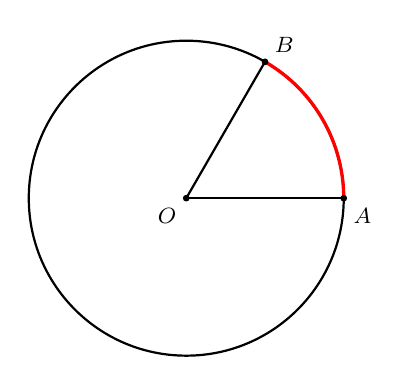
\begin{tikzpicture}[scale=1, font=\footnotesize, line join=round, line cap=round, >=stealth]
			% Vẽ đường tròn tâm O bán kính 3cm
			\draw[thick] (0,0) circle(2);
			% Gán tọa độ
			\coordinate (O) at (0,0);
			\coordinate (A) at (2,0); % điểm A nằm bên phải O
			\coordinate (B) at (60:2); % điểm B tạo góc 60 độ với trục Ox
			% Tô màu đỏ cung nhỏ AB
			\draw[very thick, red] (A) arc[start angle=0, end angle=60, radius=2];
			% Vẽ bán kính OA và OB
			\draw[thick] (O) -- (A);
			\draw[thick] (O) -- (B);
			% Đánh dấu điểm
			\filldraw (O) circle (1pt) node[below left] {$O$};
			\filldraw (A) circle (1pt) node[below right] {$A$};
			\filldraw (B) circle (1pt) node[above right] {$B$};
		\end{tikzpicture}
	\end{center}
	%Lưu ý 1
	\begin{luuy}
		Để dễ ghi nhớ và suy ra được công thức tính $l$, ta có thể dùng quy tắc \lq\lq tam suất\rq\rq~như sau:
		$$\dfrac{C}{l}=\dfrac{360^\circ}{n^\circ}$$
		Từ đó, có thể tính ra được một trong ba đại lượng $C,l,n$ nếu biết hai đại lượng còn lại.\\
	\end{luuy}
	%Nhận xét 1 
	\begin{nx}
		\begin{enumerate}
			\item Hai đại lượng $l$ và $n^\circ$ là tỷ lệ thuận.
			\item Trong tường hợp hai đường tròn đồng tâm có bán kính là $R$ và $R'$, chiều dài hai cung tròn có cùng số đo thuộc hai đường tròn sẽ tỷ lệ với hai bán kính. Tức là $$\dfrac{l_{AB}}{l_{A'B'}}=\dfrac{R}{R'}$$  \begin{center}
				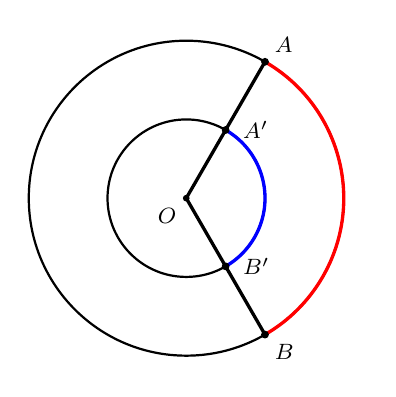
\begin{tikzpicture}[scale=1, font=\footnotesize, line join=round, line cap=round, >=stealth]
					% Tâm O
					\coordinate (O) at (0,0);
					% Bán kính
					\def\Rlarge{2}
					\def\Rsmall{1}
					% Góc tọa độ điểm A và B
					\def\angleA{60}
					\def\angleB{300}
					% Tọa độ các điểm
					\coordinate (A) at ({\Rlarge*cos(\angleA)}, {\Rlarge*sin(\angleA)});
					\coordinate (B) at ({\Rlarge*cos(\angleB)}, {\Rlarge*sin(\angleB)});
					\coordinate (A') at ({\Rsmall*cos(\angleA)}, {\Rsmall*sin(\angleA)});
					\coordinate (B') at ({\Rsmall*cos(\angleB)}, {\Rsmall*sin(\angleB)});
					% Vẽ hai đường tròn đồng tâm
					\draw[thick] (O) circle (\Rlarge);
					\draw[thick] (O) circle (\Rsmall);
					% Tô màu cung AB trên đường tròn lớn
					\draw[very thick, red] (A) arc[start angle=\angleA, end angle=-\angleA, radius=\Rlarge];
					% Tô màu cung CD trên đường tròn nhỏ
					\draw[very thick, blue] (A') arc[start angle=\angleA, end angle=-\angleA, radius=\Rsmall];	
					% Vẽ các điểm
					\filldraw (A) circle (1.2pt) node[above right] {$A$};
					\filldraw (B) circle (1.2pt) node[below right] {$B$};
					\filldraw (A') circle (1.2pt) node[right] {~$A'$};
					\filldraw (B') circle (1.2pt) node[right] {~$B'$};
					\filldraw (O) circle (1pt) node[below left] {$O$};
					%
					\draw[very thick] (O) -- (A);
					\draw[very thick] (O) -- (B);
				\end{tikzpicture}
			\end{center}
		\end{enumerate}
	\end{nx}
\end{tomtat}
%Ví dụ 1 
\begin{vd}%[Dự án EX-9-Đề Cương Toán 9]%[BUI NHI]%[9H2N4-1]
	Hoàn thành bảng sau đây (xem $\pi\approx 3{,}14$ và làm tròn kết quả đến hàng phần chục).\\
	\begin{center}
		\begin{tabular}{|c|c|c|c|c|}%|m{1cm}|m{1cm}|m{1cm}|m{1cm}|m{1cm}|}
		\hline
		\textbf{STT}&\textbf{$R$}&$C$&$n^\circ $&$l$\\
		\hline
		$1$&$9$&&$90^\circ$&\\
		\hline
		$2$&&&$60^\circ$&$40{,}6$\\
		\hline
		$3$&$22$&&&$30{,}8$\\
		\hline
	\end{tabular}
\end{center}
\loigiai{
	\begin{center}
		\begin{tabular}{|c|c|c|c|c|}%|m{1cm}|m{1cm}|m{1cm}|m{1cm}|m{1cm}|}
		\hline
		\textbf{STT}&\textbf{$R$}&$C$&$n^\circ $&$l$\\
		\hline
		$1$&$9$&$56{,}5$&$90^\circ$&$14{,}1$\\
		\hline
		$2$&$38{,}8$&$243{,}7$&$60^\circ$&$40{,}6$\\
		\hline
		$3$&$22$&$138{,}2$&$80{,}2^\circ$&$30{,}8$\\
		\hline
	\end{tabular}
\end{center}
\begin{enumerate}
	\item Chu vi của đường tròn là $C=2\pi  R=2\cdot 3{,}14\cdot9=56{,}5$.\\
	Độ dài cung tròn là $l=\dfrac{\pi R n}{180}=\dfrac{3{,}14\cdot9\cdot90}{180}=14{,}1$.
	\item Bán kính đường tròn là  $R=\dfrac{180\cdot l}{\pi n}=\dfrac{40{,}6\cdot180}{60\cdot 3{,}14}=38{,}8$.\\
	Chu vi của đường tròn là $C=2\pi R=2\cdot3{,}14\cdot38{,}8=243{,}7$.
	\item Chu vi đườnglà tròn là $C=2\pi R=2\cdot3{,}14\cdot22=138{,}2$.\\
	Số đo của cung tròn là  $n=\dfrac{360\cdot  l}{C}=\dfrac{30{,}8\cdot360}{138{,}2}=80{,}2^\circ$.
\end{enumerate}
}
\end{vd}
%Ví dụ 2 
\begin{vd}%[Dự án EX-9-Đề Cương Toán 9]%[BUI NHI]%[9H2N4-1]
Lấy $\pi\approx 3{,}14$ và làm tròn kết quả đến hàng phần trăm. Hãy tính
\begin{enumerate}
\item 
Độ dài cung tròn số đo $60^\circ$ của đường tròn đường kính $d=3$ dm.
\item Tính chu vi vành bánh xe đạp có đường kính $60$ cm.
\end{enumerate}
\loigiai{
\begin{enumerate}
	\item Bán kính của vành bánh xe là  $R=\dfrac{d}{2}=\dfrac{3}{2}=1{,}5$ (dm),\\
	Độ dài cung tròn là $l=\dfrac{\pi R n }{180}=\dfrac{3{,}14\cdot1{,}5\cdot60}{180}=1{,}57$ (dm).
	\item Chu vi vành bánh xe là $C=d\pi=60\cdot3{,}14=188{,}4$ (cm).
	\end{enumerate}}
\end{vd}
\subsubsection{Bài tập}
%\textbf{\textit{A. ĐỘ DÀI CUNG TRÒN}}
\textbf{\textit{Phần I: Trắc nghiệm nhiều lựa chọn. Khoanh tròn chữ cái A, B, C, D đứng trước đáp án mà bạn cho là đúng. }}
% Câu 1
\begin{ex}%[Dự án EX-9-Đề Cương Toán 9]%[BÙI NHI]%[9H2N4-1]
Cung tròn có số đo $n^\circ$ thuộc đường tròn $(O;R)$ có độ dài tính bởi công thức
\choice
{$l=\dfrac{\pi R n}{360}$}
{$l=\dfrac{\pi R^2 n}{360}$}
{\True $l=\dfrac{\pi R n}{180}$}
{$l=\dfrac{\pi R^2 n}{180}$}
\loigiai{Công thức tính độ dài cung tròn có số đo $n^\circ$ là $l=\dfrac{\pi R n}{180}$.}
\end{ex}
% Câu 2
\begin{ex}%[Dự án EX-9-Đề Cương Toán 9]%[BÙI NHI]%[9H2N4-1]
Trong đường tròn tâm $(O)$ bán kính $R=2$ cm, độ dài cung tròn có số đo $60^\circ$ là
\choice
{\True $\dfrac{2\pi}{3}$ cm}
{$\dfrac{4\pi}{3}$ cm}
{$\dfrac{\pi}{3}$ cm}
{$\dfrac{\pi}{6}$ cm}
\loigiai{Độ dài cung tròn có số đo $60^\circ$ là
$$l=\dfrac{\pi R n}{180}=\dfrac{\pi \cdot 2\cdot 60}{180}=\dfrac{2\pi}{3}\mathrm{~cm}.$$ }
\end{ex}
% Câu 3
\begin{ex}%[Dự án EHX-9-Đề Cương Toán 9]%[BÙI NHI]%[9H2H4-1]
Một cung tròn có số đo $60^\circ$ và chiều dài là $4\pi$ cm. Cung tròn này thuộc đường tròn có đường kính là
\choice
{$\sqrt{6}$ cm}
{$6$ cm}
{$12$ cm}
{\True $24$ cm}
\loigiai{Chiều dài cung tròn được tính theo công thức $l=\dfrac{\pi R n}{180}$\\
Suy ra $R=\dfrac{180\cdot l}{n\pi}=\dfrac{180\cdot 4\pi}{60\pi}=12$ cm. Vậy đường kính là $d=2R=24$ (cm).}
\end{ex}
% Câu 4
\begin{ex}%[Dự án EX-9-Đề Cương Toán 9]%[BÙI NHI]%[9H2H4-1]
\immini{Dựa vào hình vẽ, biết $BC=4$ cm và $AB=2$ cm. Độ dài cung tròn nhỏ $AC$ là 
\choice
{$\dfrac{2\pi}{3} $}
{\True $\dfrac{4\pi}{3} $}
{$\dfrac{\pi}{3} $}
{$\pi$}}{
\begin{tikzpicture}[scale=1, font=\footnotesize, line join=round, line cap=round, >=stealth]
	% Tâm O và đường tròn bán kính 2cm
	\coordinate (O) at (0,0);
	\draw[thick] (O) circle (2);
	% Vẽ điểm A và B sao cho AB = 2cm
	% Giả sử A nằm tại góc 150 độ trên đường tròn
	\coordinate (A) at ({2*cos(120)}, {2*sin(120)});
	% B nằm cách A 2cm trên đường tròn — chọn sao cho AB = 2cm
	% Giả sử lấy B ở góc 30 độ
	\coordinate (B) at ({2*cos(60)}, {2*sin(60)});
	% Điểm C đối xứng với B qua O
	\coordinate (C) at ($2*(O)-1*(B)$);
	% Vẽ các đoạn thẳng AB, OC, BC, AO
	\draw[thick] (A) -- (B) node[midway, below] {$2$ cm};
	\draw[thick] (A) -- (O);
	\draw[thick] (B) -- (C) node[midway, right] {$4$ cm};
	% Vẽ điểm
	\fill (O) circle (1.5pt) node[left] {$O$};
	\fill (A) circle (1.5pt) node[above left] {$A$};
	\fill (B) circle (1.5pt) node[above right] {$B$};
	\fill (C) circle (1.5pt) node[below left] {$C$};
	\end{tikzpicture}}
	\loigiai{ Xét $\Delta OAB$ có $AB=OB=OA=2$ cm. Suy ra $\Delta OAB$ là tam giác đều, do đó $\widehat{ABO}=60^\circ$.\\
Vì $\widehat{ABO}$ là góc nội tiếp chắn cung nhỏ $AC$, 
nên ta có sđ$\wideparen{AC}=2\cdot \widehat{ABO}=2\cdot 60^\circ=120^\circ $.\\
Độ dài cung nhỏ $AC$ là $l_{AC}=\dfrac{\pi R n_{AC}}{180}=\dfrac{\pi\cdot 2 \cdot 120}{180}=\dfrac{4\pi}{3}$ (cm). }
\end{ex}
% Câu 5
\begin{ex}%[Dự án EX-9-Đề Cương Toán 9]%[BÙI NHI]%[9H2H4-1]
Biết rằng cung tròn $AB$ thuộc đường tròn $(O;2\mathrm{~cm})$ có độ dài là $\pi$ cm. Độ dài dây cung $AB$ là 
\choice
{$\sqrt{2}$ cm}
{\True $2\sqrt{2}$ cm}
{$3\sqrt{2}$ cm}
{$4\sqrt{2}$ cm}
\immini{\loigiai{
	Độ dài cung tròn $AB$ tính bởi công thức $l=\dfrac{\pi R n}{180}$.\\
Suy ra $n=\dfrac{180\cdot l}{\pi R}=\dfrac{180\cdot \pi}{\pi \cdot 2}=90^\circ$.\\
	Do đó $\Delta OAB$ vuông cân tại $O$. \\
	Độ dài dây cung $AB$ là $AB=\sqrt{OA^2+OB^2}=\sqrt{2^2+2^2}=2\sqrt{2}$ (cm).}}{
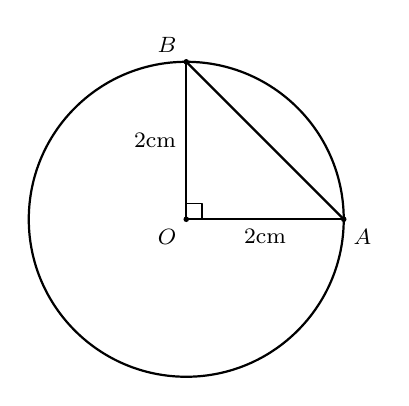
\begin{tikzpicture}[scale=1, font=\footnotesize, line join=round, line cap=round, >=stealth]
	% Tâm O và đường tròn bán kính 2cm
	\coordinate (O) at (0,0);
	\draw[thick] (O) circle (2);
	% Vẽ bán kính OA theo trục Ox (góc 0 độ)
	\coordinate (A) at (2,0);
	% Vẽ bán kính OB vuông góc với OA => góc 90 độ
	\coordinate (B) at (0,2);
	% Vẽ các bán kính
	\draw[thick] (O) -- (A) node[midway, below] {$2$cm};
	\draw[thick] (O) -- (B) node[midway, left] {$2$cm};
	\draw[thick] (A) -- (B);
	% Đánh dấu vuông góc tại O
	\draw (0.2,0) -- (0.2,0.2) -- (0,0.2);
	% Vẽ các điểm
	\fill (O) circle (1pt) node[below left] {$O$};
	\fill (A) circle (1pt) node[below right] {$A$};
	\fill (B) circle (1pt) node[above left] {$B$};
	\end{tikzpicture}}
\end{ex}
\textbf{\textit{Phần II: Tự  luận}} 
% Bài 1
\begin{bt}%[Dự án EX-9-Đề Cương Toán 9]%[BÙI NHI]%[9H2V4-1]
Một thợ cơ khí cần làm lan can bao quanh một đoạn cong của sân thượng, hình cung tròn có bán kính $2{,}5$ m, và góc ở tâm là $150^\circ$.
\begin{enumerate}
\item Tính chiều dài lan can cần làm.
\item  Nếu mỗi đoạn lan can dài $1{,}2$ m, người thợ cần ít nhất bao nhiêu đoạn để ghép lại?
\end{enumerate}
\loigiai{
\begin{enumerate}
	\item Chiều dài lan can cần làm $l=\dfrac{\pi R n}{180}=\dfrac{\pi \cdot 2{,}5 \cdot 150 }{180}=\dfrac{25\pi}{12}$ (m).
	\item  Ta có $\dfrac{25\pi}{12} \colon 1{,}2 \approx 5{,}45$ (m). 
	Vậy với mỗi đoạn lan can là $1{,}2$ m thì cần ít nhất $6$ đoạn lan can. 
	\end{enumerate}}
\end{bt}
% Bài 2
\begin{bt}%[Dự án EX-9-Đề Cương Toán 9]%[BÙI NHI]%[9H2V4-1]
Một nhóm học sinh thiết kế mô hình tàu lượn mini. Một đoạn ray của tàu là $\dfrac{1}{4}$ vòng tròn có bán kính $0{,}8$ m.
\begin{enumerate}
\item Tính chiều dài đoạn ray cong.
\item  Nếu muốn mở rộng mô hình với cung tròn $180^\circ$, cần bao nhiêu ray loại đó để ghép đủ?
\end{enumerate}
\loigiai{
\begin{enumerate}
	\item $\dfrac{1}{4}$ đường tròn có số đo là $90^\circ$. Chiều dài của đường ray là $l=\dfrac{\pi R n}{180}=\dfrac{\pi \cdot 0{,}8\cdot 90}{180}=\dfrac{2\pi}{5}$ (m).
	\item  Nếu muốn mở rộng mô hình với cung tròn $180^\circ$, chiều dài đường ray là $l=2\cdot\dfrac{2\pi}{5}=\dfrac{4\pi}{5}$ (m). \\Vậy cần hai đoạn đường ray.
	\end{enumerate}}
\end{bt}
% Bài 3
\begin{bt}%[Dự án EX-9-Đề Cương Toán 9]%[BÙI NHI]%[9H2V4-1]
Cho đường tròn $(O)$ bán kính $OA$. Từ trung điểm $M$ của $OA$ vẽ dây $BC \perp OA$. Biết độ dài đường tròn $(O)$ là $4\pi$ cm. Tính
\begin{enumerate}
\item Bán kính đường tròn $(O)$,
\item Độ dài hai cung nhỏ và cung lớn $BC$ của đường tròn.
\end{enumerate}
\immini{\loigiai{Độ dài đường tròn $(O)$ là $4\pi$ cm, tức là $C=4\pi$ (cm)
	\begin{enumerate}
		\item Bán kính của đường tròn $(O)$ là $R=\dfrac{C}{2\pi}=\dfrac{4\pi}{2\pi}=2$  (cm);
		\item Ta có $OM=MA=\dfrac{1}{2}OA=1$ cm (giả thiết $M$ là trung điểm $OA$). Do đó $\cos\left(\widehat{MOB} \right)=\dfrac{OM}{OB}=\dfrac{1}{2}$, suy ra $\widehat{AOB}=~60^\circ$, suy ra $\widehat{COB}=120^\circ $. Vì $\widehat{COB}$ là góc ở tâm chắn cung nhỏ $BC$ nên sđ$ \wideparen{BC}=120^\circ$.\\ Độ dài cung nhỏ $BC$ là $l=\dfrac{\pi R n}{180}=\dfrac{\pi\cdot2\cdot120}{180}=\dfrac{4\pi}{3}$  (cm).\\
		Độ dài cung lớn $BC$$\colon$ $4\pi-\dfrac{4\pi}{3}=\dfrac{8\pi}{3}$ (cm).
		\end{enumerate}	}}
		{\begin{tikzpicture}[scale=1, font=\footnotesize, line join=round, line cap=round, >=stealth]
	% Tâm và bán kính
	\coordinate (O) at (0,0);
	\coordinate (A) at (2,0);
	\coordinate (M) at ($(O)!0.5!(A)$); % Trung điểm OA
	
	% Dựng đường tròn tâm O, bán kính 2
	\draw [thick] (O) circle (2cm);
	% Vẽ đoạn OA và điểm M
	\draw [thick] (O) -- (A);
	\fill (O) circle (0.5pt) node[below left] {$O$};
	\fill (A) circle (0.5pt) node[right] {$A$};
	\fill (M) circle (0.5pt) node[below right] {$M$};
	% Dựng dây BC vuông góc với OA tại M
	\draw [thick] (O) -- ++(60:2cm) coordinate (B);
	\draw [thick] (O) -- ++(-60:2cm) coordinate (C);
	\draw [thick] (B) -- (C);
	\fill (B) circle (0.5pt) node[above] {$B$};
	\fill (C) circle (0.5pt) node[below] {$C$};
	% Đánh dấu vuông góc tại M
	\draw (M)++(0.1,0) --++(0,0.1) --++(-0.1,0);
	\draw (0.9,0.9) -- (1.1,1.1);
	\draw (0.9,-0.9) -- (1.1,-0.7);
	\end{tikzpicture}}
\end{bt}
% Bài 4
\begin{bt}%[Dự án EX-9-Đề Cương Toán 9]%[BÙI NHI]%[9H2V4-1]
Cho tam giác $ABC$ có $AB=AC=3$ cm và $\widehat{A}=120^\circ$. Tính độ dài đường tròn ngoại tiếp tam giác $ABC$.
\loigiai{
\immini{Gọi $O$ là tâm đường tròn ngoại tiếp $\Delta ABC$.\\ Vì $\Delta ABC$ cân tại $A$ và $\widehat{A}=120^\circ$ nên $\widehat{CBA}=\widehat{BCA}=30^\circ$\\
	Mà $\widehat{CBA}$ là góc nội tiếp chắn cung tròn nhỏ $AC$ nên,\\
	ta có $\text{sđ}\wideparen{AC}=2 \cdot \widehat{CBA}=2\cdot 30^\circ=60^\circ$\\
	Xét $\Delta OAC$, ta có $\Delta OAC$ cân tại $O$ và $\widehat{AOC}=\text{sđ}\wideparen{AC}=60^\circ$\\(góc ở tâm chắn cung nhỏ $AC$). Do đó $\Delta OAC$ là tam giác đều, ta có $AC=OA=OC=R=3$ cm.\\
	Độ dài đường tròn $(O)$ cũng chính là chu vi của đường tròn.
	$$C=2\pi  R =2\cdot \pi \cdot 3 =6\pi \left( \mathrm{cm}\right).$$}{
	\begin{tikzpicture}[scale=1, font=\footnotesize, line join=round, line cap=round, >=stealth]
		% Tâm O và bán kính
		\coordinate (O) at (0,0);
		\def\r{3}
		
		% Đặt A tại góc 0 độ (phải)
		\coordinate (A) at ({\r*cos(0)}, {\r*sin(0)});
		
		% B và C cách A ±120 độ quanh đường tròn
		\coordinate (B) at ({\r*cos(60)}, {\r*sin(60)});
		\coordinate (C) at ({\r*cos(60)}, {\r*sin(-60)});
		\
		% Vẽ đường tròn
		\draw[red, dashed] (O) circle (\r);
		\node at (O) [below left] {$O$};
		
		% Vẽ tam giác ABC
		\draw[thick] (A) -- (B) -- (C) -- cycle;
		\draw[thick] (A) -- (O) -- (C)-- cycle;
		% Nhãn các đỉnh
		\node[right] at (A) {$A$};
		\node[above] at (B) {$B$};
		\node[below] at (C) {$C$};
		
		% Ký hiệu góc A = 120 độ
		\draw pic["$120^\circ$", draw=black, angle radius=3.5mm, angle eccentricity=1.8, text=black,
		pic text={$\scriptstyle 120^\circ$},  
		pic text options={xshift=2pt, yshift=4pt}] {angle = B--A--C};
		\draw pic[draw=black, angle radius=5mm, angle eccentricity=1.3,text=black,
		pic text={$\scriptstyle 30^\circ$}, 
		pic text options={xshift=0.5pt, yshift=-4pt}] {angle = C--B--A};
		% Ký hiệu AB = AC
		\draw ($(A)!0.5!(B)$) -- ++(60:2pt) -- ++(240:4pt);
		\draw ($(A)!0.5!(C)$) -- ++(-60:2pt) -- ++(120:4pt);5
\end{tikzpicture}}
}
\end{bt}
% Bài 5
\begin{bt}%[Dự án EX-9-Đề Cương Toán 9]%[BÙI NHI]%[9H2V4-1]
Cho hai đường tròn đồng tâm $(O)$ có bán kính lần lượt là, $R_1=3$  cm, $R_2=6$ cm. Một dây $AB$ của đường tròn $(O;R_2)$ tiếp xúc với đường tròn $(O;R_1)$ tại $C$.
\begin{enumerate}
\item Tính độ dài cung nhỏ $AB$ của đường tròn $(O,R_2)$,
\item Tính độ dài đường tròn đường kính $AB$.
\end{enumerate}
\loigiai{\immini{
	\begin{enumerate}
		\item Ta có $AB$ là một tiếp tuyến của đường tròn $(O;R_1)$, gọi $C$ là tiếp điểm của $AB$ và $(O;R_1)$, khi đó $OC \perp AB$.\\
		Tam giác $OAC$ vuông tại $A$ có $\cos\widehat{AOC}=\dfrac{OC}{OA}=\dfrac{1}{2}$.\\
		Suy ra $\widehat{AOC}=60^\circ$, do đó $\widehat{AOB}=2\cdot \widehat{AOC}=120^\circ=\text{sđ}\wideparen{AB}$.\\
		Độ dài cung nhỏ $AB$ thuộc đường tròn $(O,R_2)$ là $$l_{AB}=\dfrac{\pi R n_{AB}}{180}=\dfrac{\pi \cdot 6 \cdot 120}{180}=4\pi\left(\mathrm{cm}\right).$$
		\item Vì $\Delta OCA$ vuông tại $C$ nên theo định lý Pythagoras\\ $AC =\sqrt{R_2^2-R_1^2}= \sqrt{6^2-3^2}=3\sqrt{3}$.\\
		$AB$ nằm trên tiếp tuyến của $(O,R_1)$ tại tiếp điểm $C$,\\ nên $OC \perp AB$ tại $C$. Suy ra $C$ là trung điểm của $AB$. \\Do đó $AB=2\cdot AC =2\cdot 3\sqrt{3}=6\sqrt{3}$\\
		Độ dài đường tròn (chu vi đường tròn) đường kính $AB$ là 
		$$C=d\pi=AB\cdot\pi=6\pi\sqrt{3}\left(\mathrm{cm}\right).$$
\end{enumerate}}{
	\begin{tikzpicture}[scale=1, font=\footnotesize, line join=round, line cap=round, >=stealth]
		% Tâm O
		\coordinate (O) at (0,0);
		% Bán kính
		\def\Rone{1.5}  % R1 = 3 cm (tròn nhỏ)
		\def\Rtwo{3}  % R2 = 6 cm (tròn lớn)
		% Điểm C nằm trên đường tròn nhỏ, ta chọn trên trục Oy (vị trí đơn giản)
		\coordinate (C) at (0,\Rone);
		% Dây AB vuông góc với OC tại C, nên AB nằm ngang
		% Tính độ dài AB = 6√3, => AB/2 = 3√3 ≈ 5.2
		\def\halfAB{2.6} % gần đúng 3√3
		% Tọa độ A và B6
		\coordinate (A) at ($ (C) + (-\halfAB, 0) $);
		\coordinate (B) at ($ (C) + (\halfAB, 0) $);
		% Vẽ hai đường tròn đồng tâm
		\draw[thick, green] (O) circle (\Rone); % đường tròn nhỏ
		\draw[thick,red] (O) circle (\Rtwo);         % đường tròn lớn
		% Vẽ dây AB tiếp xúc đường tròn nhỏ tại C
		\draw[very thick, blue] (A) -- (B);
		% Vẽ các đoạn từ tâm
		\draw[thick, color=green] (O) -- (C);
		\draw[thick, color=red] (O) -- (B);
		\draw[thick, color=red] (O) -- (A);
		% Ký hiệu góc vuông tại C
		\draw ($(C)+(0.2,0)$) -- ++(0,-0.2) -- ++(-0.2,0);
		% Đặt tên các thickđiểm
		\node[below] at (O) {$O$};
		\node[above] at (C) {$C$};
		\node[left] at (A) {$A$};
		\node[right] at (B) {$B$};
		% Ghi bán kính nếu muốn
		\node[left] at ($(O)!0.5!(C)$) {\small $R_1$};
		\node[below right] at ($(O)!0.5!(B)$) {\small $R_2$};
		\end{tikzpicture}}}
\end{bt}
\subsection{Diện tích hình quạt tròn-Hình vành khuyên}
\subsubsection{Kiến thức trọng tâm}
%lý thuyết Diện tích hình quạt tròn
\begin{boxdn}
\begin{itemize}
\item \textbf{Hình quạt tròn} $OAB$ là hình giới hạn bởi một cung tròn $\wideparen{AB}$ và hai bán kính $OA,OB$.
\item Diện tích của một hình tròn tâm $O$, bán kính $R$ là 
$$S=\pi R^2.$$
\item Diện tích hình quạt tròn $OAB$ với cung tròn $\wideparen{AB}$ có số đo $n^\circ$ trên đường tròn $\left(O;R \right)$, ký hiệu là $S_q$ và được tính bằng công thức $$S_q=\dfrac{\pi  R^2  n}{360}.$$
\item \textbf{Hình vành khuyên} là hình được giới hạn bởi hai đường tròn đồng tâm.
\item Hình vành khuyên được giới hạn bởi hai đường tròn $(O;R)$ và $(O;r)$ với $(R>r)$ có diện tích tính bởi công thức 
$$S_{vk}=\pi (R^2-r^2).$$
\item \textbf{Hình viên phân} là phần hình tròn được giới hạn bởi dây cung và cung tròn có cùng hai đầu mút trên đường tròn.
\item Diện tích hình viên phân giới hạn bởi dây cung và cung nhỏ $AB$ được tính bằng cách lấy hiệu số  \textbf{\textit{diện tích hình quạt tròn}} $OAB$ và \textbf{\textit{diện tích tam giác}} $OAB$.
\end{itemize}
\end{boxdn}
% Hình quạt tròn
\begin{minipage}{0.45\textwidth}
\begin{center}
\begin{tikzpicture}[scale=1, font=\footnotesize, line join=round, line cap=round, >=stealth]
	% Tọa độ các điểm
	\coordinate (O) at (0,0);
	\coordinate (A) at (2,0);% điểm A trên trục hoành
	\coordinate (B) at (60:2);% điểm B tạo góc 60 độ với Ox, bán kính 3cm
	% Tô màu hình quạt tròn OAB bằng màu nâu nhạt
	\fill[fill=brown!20] (O) -- (A) arc[start angle=0, end angle=60, radius=2cm] -- cycle;
	% Vẽ đường tròn (chỉ phần viền ngoài)
	\draw[thick] (O) circle(2cm);
	% Vẽ hai bán kính OA và OB
	\draw[thick] (O) -- (A);
	\draw[thick] (O) -- (B);
	% Đánh dấu các điểm
	\filldraw (O) circle (1pt) node[below left] {$O$};
	\filldraw (A) circle (1pt) node[below right] {$A$};
	\filldraw (B) circle (1pt) node[above right] {$B$};
	\draw (0,-2) circle (0pt) node[below] {$\text{Hình quạt tròn OAB}$};
\end{tikzpicture}
\end{center}
\end{minipage}
\hfill
%Hình vành khuyên
\begin{minipage}{0.45\textwidth}
\begin{center}
\begin{tikzpicture}[scale=1, font=\footnotesize, line join=round, line cap=round, >=stealth]
	\draw [line width=1pt,color=black,fill=red,fill opacity=1] (0,0) circle (2cm);
	\draw [line width=1pt,color=black,fill=white,fill opacity=1] (0,0) circle (1.5cm);
	\begin{scriptsize}
		\draw [fill=black] (0,0) circle (1pt);1
		\draw[color=black] (0,-0.5) node {$O$};
	\end{scriptsize}
	\draw (0,-2) circle (0pt) node[below] {$\text{Hình vành khuyên}$};
\end{tikzpicture}
\end{center}
\end{minipage}
%Hình viên phân 	
\begin{center}
\begin{tikzpicture}[scale=1, font=\footnotesize, line join=round, line cap=round, >=stealth]
% Tâm và bán kính
\coordinate (O) at (0,0);
\draw [line width=1pt,color=black,fill=white,fill opacity=1] (0,0) circle (2cm);
\def\r{2} % bán kính
% Điểm A và B cách nhau 60 độ trên đường tròn
\coordinate (A) at ({\r*cos(130)}, {\r*sin(130)});
\coordinate (B) at ({\r*cos(50)}, {\r*sin(50)});
% Cung tròn nhỏ AB (góc ở tâm 60 độ)
\draw[thick] (A) arc[start angle=130, end angle=50, radius=\r];
% Dây cung AB
\draw[thick] (A) -- (B);
% Tâm O và các đoạn OA, OB
\draw[thick] (O) -- (A);
\draw[thick] (O) -- (B);
% Điểm đánh dấu
\fill (O) circle (1pt) node[below] {$O$};
\fill (A) circle (1pt) node[above left] {$A$};
\fill (B) circle (1pt) node[above right] {$B$};
% Ghi bán kính
%\node at ($(O)!0.5!(A)$) [below left] {$3\,\text{cm}$};
% Ghi độ cung
\draw pic[draw=black, angle radius=0.5cm, angle eccentricity=1.5] {angle=B--O--A};
% Tô màu vùng viên phân
\begin{scope}
	\fill[blue!80, opacity=0.5] (A) arc[start angle=130, end angle=50, radius=\r] -- (B) -- cycle;
\end{scope}
\draw (0,-2) circle (0pt) node[below] {$\text{Hình viên phân giới hạn bởi dây cung $AB$ và cung nhỏ AB.}$};
\end{tikzpicture}
\end{center}
%Lưu ý 2
\begin{luuy}
Để dễ ghi nhớ và suy ra được công thức tính $S_q$, ta có thể dùng quy tắc \lq\lq tam suất\rq\rq~như sau:
$$\dfrac{S}{S_q}=\dfrac{360^\circ}{n^\circ}$$
Từ đó, có thể tính ra được một trong ba đại lượng $S_q,S,n$ nếu biết hai đại lượng còn lại.
\end{luuy}
%Ví dụ 3
\begin{vd}%[Dự án EX-9-Đề Cương Toán 9]%[BÙI NHI]%[9H2N4-2]
Lấy giá trị gần đúng của $\pi \approx 3{,}14$, hãy điền vào ô trống trong bảng sau (đơn vị độ dài$\colon$ cm, làm tròn kết quả đến chữ số thập phân thứ hai).
\begin{center}
\begin{tabular}{|c|c|c|c|c|c|}%|m{1cm}|m{1cm}|m{1cm}|m{1cm}|m{1cm}|m{1cm}|}
\hline
\textbf{STT}&\textbf{$R$}&$C$&$S$&$n^\circ $&$S_q$\\
\hline
$1$&$3$&&&$60^\circ$&\\
\hline
$2$&&$15{,}7$&&$80^\circ$&\\
\hline
$3$&&&$50{,}24$&&$6{,}28$\\
\hline
\end{tabular}
\end{center}
\loigiai{
\begin{center}
\begin{tabular}{|c|c|c|c|c|c|}%|m{1cm}|m{1cm}|m{1cm}|m{1cm}|m{1cm}|m{1cm}|}
\hline
\textbf{STT}&\textbf{$R$}&$C$&$S$&$n^\circ $&$S_q$\\
\hline
$1$&$3$&$18{,}84$&$28{,}26$&$60^\circ$&$4{,}71$\\
\hline
$2$&$2{,}5$&$15{,}7$&$19{,}63$&$80^\circ$&$4{,}36$\\
\hline
$3$&$4$&$25{,}12$&$50{,}24$&$45^\circ$&$6{,}28$\\
\hline
\end{tabular}
\end{center}
\begin{enumerate}
\item Chu vi đường tròn $C=2\pi R=2\cdot \pi \cdot 3=6\pi = 18{,}84$ (cm),\\
Diện tích hình tròn $S=\pi R^2=\pi \cdot 3^2=9\pi= 28{,}26$ (cm$^2$),\\
Diện tích hình quạt $S_q=\dfrac{\pi R^2 n}{360}=\dfrac{\pi \cdot 3^2 \cdot 60}{360}= 4{,}71$ (cm$^2$).
\item Chu vi đường tròn $C=2\pi R=15{,}7$, suy ra $R=\dfrac{C}{2\pi}=\dfrac{15{,}7}{2\cdot 3{,}14}= 2{,}5$ (cm),\\
Diện tích hình tròn $S=\pi R^2=\pi \cdot 2{,}5^2=6{,}25\pi= 19{,}63$ (cm$^2$),\\
Diện tích hình quạt $S_q=\dfrac{\pi R^2 n}{360}=\dfrac{\pi \cdot 2{,}5^2 \cdot 80}{360}= 4{,}36$ (cm$^2$).
\item 	Diện tích hình tròn $S=\pi R^2$. Suy ra $R=\sqrt{\dfrac{S}{\pi} }=\sqrt{\dfrac{50{,}24}{3{,}14}}=4$ (cm$^2$),\\
Chu vi đường tròn $C=2\pi R=2\cdot 3{,}14 \cdot 4=25{,}12$ (cm),\\
Diện tích hình quạt $S_q=\dfrac{\pi R^2 n}{360}$, suy ra $n=\dfrac{S_q\cdot 360}{\pi R^2}=\dfrac{6{,}28 \cdot 360}{3{,}14\cdot 4^2}=45^\circ$.
\end{enumerate}}
\end{vd}
%Nhận xét 2 
\begin{nx}
Dựa vào công thức của diện tích hình quạt và chiều dài cung tròn tương ứng ta có các mối liên hệ sau đây
\begin{enumerate}
\item Diện tích hình quạt $OAB$, $S_q$ và chiều dài cung tròn nhỏ $ AB$, $l_{AB}$ là hai đại lượng tỷ lệ thuận, cụ thể là \begin{center}
$S_q=\dfrac{R}{2}\cdot l_{AB}$ (với $R$ là bán kính đường tròn).
\end{center}
\item Diện tích hình quạt tròn $S_q$ và số đo cung tròn $n^\circ$ là hai đại lượng tỷ lệ thuận.
\item Vì hình vành khuyên được tạo bởi hai đường tròn đồng tâm nên \lq\lq\textit{\textbf{Hình quạt vành khuyên}}\rq\rq~được tạo bởi hai cung tròn có số đo $n^\circ$ thuộc hai đường tròn (có bán kính là $R$, $r$) và hai bán kính của đường tròn lớn, có thể được tính diện tích bằng công thức $$S_{qvk}=\dfrac{\pi n}{360}\left(R^2-r^2 \right).$$
\begin{center}
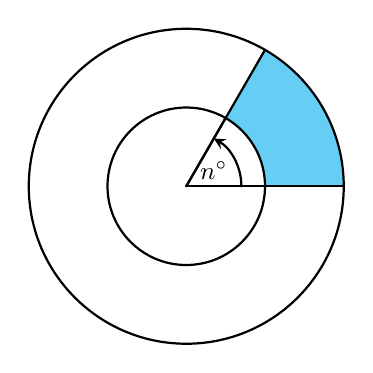
\begin{tikzpicture}[scale=1, font=\footnotesize, line join=round, line cap=round, >=stealth]
% Bán kính trong và ngoài
\def\rinner{1}
\def\router{2}
\def\angle{60} % số đo góc quạt (độ)
% Tô phần hình quạt vành khuyên
\fill[cyan!60] 
(0,0) -- (\angle:\rinner) 
arc[start angle=\angle, end angle=0, radius=\rinner] 
-- (0:\router)
arc[start angle=0, end angle=\angle, radius=\router]
-- cycle;
% Vẽ đường tròn ngoài
\draw[thick] (0,0) circle (\router);
% Vẽ đường tròn trong
\draw[thick] (0,0) circle (\rinner);
% Vẽ hai bán kính
\draw[thick] (0,0) -- (0:\rinner);
\draw[thick] (0,0) -- (\angle:\rinner);
\draw[thick] (0,0) -- (0:\router);
\draw[thick] (0,0) -- (\angle:\router);
% Ghi nhãn góc
\draw[->, thick] (0.7,0) arc[start angle=0, end angle=60, radius=0.7];
\node at (0.35,0.2) {\small $n^\circ$};
\end{tikzpicture}
\end{center}
\item Từ nhận xét thứ $2$, ta cũng có số đo hình quạt vành khuyên $n^\circ$ và diện tích của nó (qvk) $S_{qvk}$ là hai đại lượng tỷ lệ thuận, hay ta có
$$\dfrac{S_{qvk}}{n}=\dfrac{S_{vk}}{360}.$$
\end{enumerate}	
\end{nx}
\subsubsection{Bài tập}
\textbf{\textit{Phần I: Trắc nghiệm nhiều lựa chọn. Khoanh tròn chữ cái A, B, C, D đứng trước đáp án mà bạn cho là đúng. }}
% Câu 6
\begin{ex}%[Dự án EX-9-Đề Cương Toán 9]%[BÙI NHI]%[9H2N4-2]
Cho đường tròn $(O; 2\mathrm{~cm})$, vẽ dây cung $BC=2\sqrt{3}$ cm và bán kính $OA \perp BC$ tại $M$. Diện tích của hình quạt tròn $BOC$ là  
\choice
{$\dfrac{2\pi}{3}$ cm}
{\True $\dfrac{4\pi}{3}$ cm}
{$\dfrac{\pi}{3}$ cm}
{$\dfrac{\pi}{3}$ cm}
\immini{\loigiai{Vì $OA \perp BC$ tại $M$, theo tính chất giữa đường kính và dây cung thì $M$\\
là trung điểm của $BC$. Ta có $MB=MC=\sqrt{3}$\\
Xét $\Delta OMC$ vuông tại $M$, ta có $\sin\widehat{COM} =\dfrac{MC}{OC}=\dfrac{\sqrt{3}}{2}$,\\
suy ra $\widehat{COM}=60^\circ$, do đó $\widehat{BOC}=120^\circ$. \\
Hơn nữa vì $\widehat{BOC}$ là góc ở tâm chắn cung $BAC$ nên $\text{sđ}\wideparen{BAC}=120^\circ$.\\
Diện tích hình quạt tròn $BOC$ là $S_q=\dfrac{\pi R^2 n}{360}=\dfrac{\pi \cdot 2^2 \cdot 120}{360}=\dfrac{4\pi}{3}$ (cm$^2$).}}{
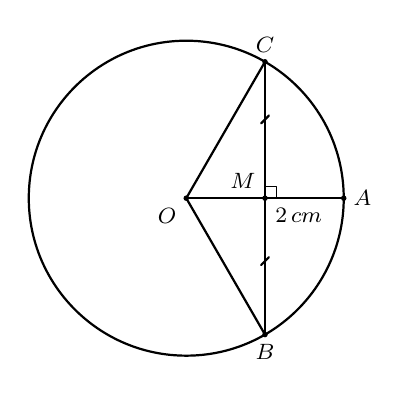
\begin{tikzpicture}[scale=1, font=\footnotesize, line join=round, line cap=round, >=stealth]
% Tâm và bán kính
\coordinate (O) at (0,0);
\def\r{2} % bán kính
% Điểm A trên đường tròn, chọn phía trên
\coordinate (A) at (2,0);
\coordinate (M) at (1,0);
% Điểm D là hình chiếu của A lên BC, nằm trên đường nằm ngang qua O
\coordinate (D) at (0,0);
% BC nằm ngang, vuông góc OA tại D, độ dài BC = 2√3 => BD = DC = √3
\coordinate (C) at ({\r*cos(60)}, {\r*sin(60)});
\coordinate (B) at ({\r*cos(-60)}, {\r*sin(-60)});
% Vẽ đường tròn tâm O bán kính 2
\draw[thick] (O) circle (\r);
% Vẽ các
\draw[thick] (O) -- (A) node[midway, below right] {$2\,\text{cm}$};
\draw[thick] (O) -- (B);
\draw[thick] (O) -- (C);
\draw[thick] (B) -- (C);
\draw[thick] (0.95,0.95)--(1.05,1.05);
\draw[thick] (0.95,-0.85)--(1.05,-0.75);
% Đánh dấu vuông góc
\draw (1,0) ++(0.15,0) -- ++(0,0.15) -- ++(-0.15,0);
% Các điểm
\fill (O) circle (1pt) node[below left] {$O$};
\fill (A) circle (1pt) node[right] {$A$};
\fill (B) circle (1pt) node[below] {$B$};
\fill (C) circle (1pt) node[above] {$C$};
\fill (M) circle (1pt) node[above left] {$M$};
\end{tikzpicture}}
\end{ex}
% Câu 7
\begin{ex}%[Dự án EX-9-Đề Cương Toán 9]%[BÙI NHI]%[9H2N4-2]
Trên đường tròn $(O)$, hình quạt tròn $OAB$ có diện tích là $\dfrac{\pi}{3}$ (cm$^2$) và sđ$\wideparen{AB}=60^\circ$, diện tích của hình tròn khi đó là 
\choice
{$\dfrac{\pi}{2}$}
{$\pi$}
{\True $2\pi$}
{$4\pi$}
\loigiai{ Ta có tỷ lệ $\dfrac{S_q}{S}=\dfrac{n}{360}$, suy ra $S=\dfrac{S_q\cdot 360}{n}=\dfrac{\dfrac{\pi}{3}\cdot 360}{60}=2\pi$ (cm$^2$).}
\end{ex}
% Câu 8
\begin{ex}%[Dự án EX-9-Đề Cương Toán 9]%[BÙI NHI]%[9H2H4-2]
Cho đường tròn $(O;2\mathrm{~cm})$ và đường tròn  $(O;1\mathrm{~cm})$. Vẽ hai bán kính $OA$, $OB$ của đường tròn lớn cắt đường tròn nhỏ lần lượt tại $C$ và $D$. Tỷ số diện tích giữa hình quạt tròn $OAB$ và $COD$ là
\choice
{$\dfrac{S_{OAB}}{S_{COD}}=\dfrac{1}{2}$}
{$\dfrac{S_{OAB}}{S_{COD}}=\dfrac{1}{4}$}
{$\dfrac{S_{OAB}}{S_{COD}}=2$}
{\True $\dfrac{S_{OAB}}{S_{COD}}=4$}
\immini{\loigiai{Các góc $AOB$ và $COD$ là góc nội tiếp lần lượt chắn các cung nhỏ $AB$ và $CD$ thuộc hai đường tròn $(O;2\mathrm{~cm})$, $(O;1\mathrm{~cm})$ ($R=1$ cm, $r=2$ cm). Do đó hai hình quạt tròn $ OAB$ và $OCD$ có cùng số đo. Vậy tỷ số diện tích giữa hai hình là
$$\dfrac{S_{OAB}}{S_{OCD}}=\dfrac{\dfrac{\pi R^2  n_{AB}}{360}}{\dfrac{\pi r^2  n_{DC}}{360}}=\dfrac{R^2}{r^2}=\dfrac{2^2}{1^2}=4.$$}}{
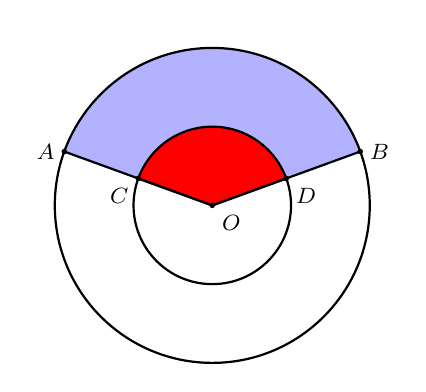
\begin{tikzpicture}[scale=1, font=\footnotesize, line join=round, line cap=round, >=stealth]
% Tâm O và bán kính
\coordinate (O) at (0,0);
\def\rsmall{1}
\def\rbig{2}
% Chọn hai điểm A và B trên đường tròn lớn (không đối xứng qua O)
\coordinate (A) at ({\rbig*cos(160)}, {\rbig*sin(160)});
\coordinate (B) at ({\rbig*cos(20)}, {\rbig*sin(20)});
\coordinate (C) at ({\rsmall*cos(160)}, {\rsmall*sin(160)});
\coordinate (D) at ({\rsmall*cos(20)}, {\rsmall*sin(20)});
% Tô màu hình quạt lớn OAB (dùng cung tròn thật)
\fill[blue!30] 
(O) -- (A)
arc[start angle=160, end angle=20, radius=2] -- cycle;
% Tô màu hình quạt nhỏ OCD (dùng cung tròn thật)
\fill[red] 
(O) -- (C)
arc[start angle=160, end angle=20, radius=1] -- cycle;
% Vẽ 2 đường tròn đồng tâm
\draw[thick] (O) circle(\rbig);
\draw[thick] (O) circle(\rsmall);
% Vẽ các đoạn thẳng
\draw[thick,] (O) -- (D);
\draw[thick,] (O) -- (C);
\draw[thick,] (O) -- (A);
\draw[thick,] (O) -- (B);
% Gán nhãn các điểm
\fill (O) circle(1pt) node[below right] {$O$};
\fill (A) circle(1pt) node[left] {$A$};
\fill (B) circle(1pt) node[right] {$B$};
\fill (C) circle(1pt) node[below left] {$C$};
\fill (D) circle(1pt) node[below right] {$D$};		
\end{tikzpicture}}
\end{ex}
% Câu 9
\begin{ex}%[Dự án EX-9-Đề Cương Toán 9]%[BÙI NHI]%[9H2N4-2]
Cho đường tròn tâm $O$, đường kính $AB=4$ cm. Biết rằng $BC=2$ cm,  hình viên phân tạo bởi dây cung và cung tròn nhỏ $BC$ có diện tích là bao nhiêu?
\choice
{\True $\sqrt{3}-\dfrac{2\pi}{3}$ (cm$^2$)}nhỏ
{$\dfrac{\sqrt{3}}{2}-\dfrac{2\pi}{3}$ (cm$^2$)}
{$\sqrt{3}-\dfrac{\pi}{3}$ (cm$^2$)}
{$\dfrac{\sqrt{3}}{2}-\dfrac{2\pi}{3}$ (cm$^2$)}
\immini{\loigiai{Gọi $M$ là trung điểm $OB$, vì $OB=OC=BC=2$ cm nên $\Delta OBC$ đều. Vẽ $CM \perp OB$ tại $M$. Ta có góc $BOC=60^\circ$. Diện tích tam giác $OBC$ là\\ $S_{\Delta OBC}=\dfrac{1}{2}\cdot OB\cdot CM=\dfrac{1}{2}\cdot OB \cdot OC\cdot\sin\widehat{BOC}=\dfrac{1}{2}\cdot 2\cdot 2\cdot\dfrac{\sqrt{3}}{2}=\sqrt{3}$.\\ 
Diện tích hình quạt $OBC$ là $S_q=\dfrac{\pi R^2 n}{360}=\dfrac{\pi \cdot 2^2 \cdot 60}{360}=\dfrac{2\pi}{3}$.\\
Vậy diện tích hình viên phân là $S=S_q-S_{\Delta OBC}=\sqrt{3}-\dfrac{2\pi}{3}$ (cm$^2$).}}{
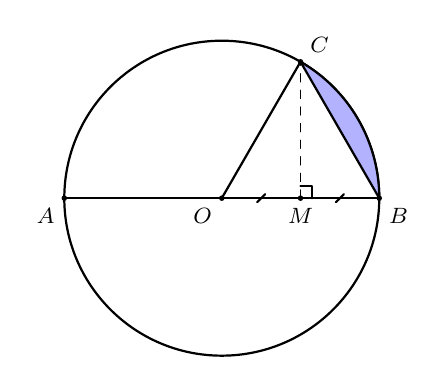
\begin{tikzpicture}[scale=1, font=\footnotesize, line join=round, line cap=round, >=stealth]
% Tâm O tại gốc, bán kính R = 2cm
\def\R{2}
\coordinate (O) at (0,0);
% Điểm A và B trên đường kính AB = 4cm
\coordinate (A) at (-2,0); 
\coordinate (B) at (2,0);
\coordinate (M) at (1,0);
\draw[thick] (A) -- (B);5
\draw[thick] (O) circle(\R);
% Đặt điểm C sao cho BC = 2 cm, nằm trên đường tròn
% Giả sử góc tại tâm từ B đến C là 60 độ (ta chọn để được BC = 2)
\coordinate (C) at ({\R*cos(60)}, {\R*sin(60)});
% Tô hình viên phân: cung BC và đoạn BC
\fill[blue!30] (B) arc[start angle=0, end angle=60, radius=\R] -- (C) -- cycle;
% Vẽ cung BC
\draw[thick] (B) arc[start angle=0, end angle=60, radius=\R];
% Vẽ đoạn thẳng BC,OC
\draw[thick] (B) -- (C);
\draw[thick] (O) -- (C);
\draw[dashed] (M) -- (C);
\draw[thick] (1,0.15)--(1.15,0.15)--(1.15,0);
\draw[thick] (0.45,-0.05)--(0.55,0.05);
\draw[thick] (1.45,-0.05)--(1.55,0.05);
% Tâm và nhãn1
\fill (O) circle(1pt) node[below left] {$O$};
\fill (M) circle(1pt) node[below] {$M$};
\fill (A) circle(1pt) node[below left] {$A$};
\fill (B) circle(1pt) node[below right] {$B$};
\fill (C) circle(1pt) node[above right] {$C$};
\end{tikzpicture}}
\end{ex}
% Câu 10
\begin{ex}%[Dự án EX-9-Đề Cương Toán 9]%[BÙI NHI]%[9H2T4-3]
\immini{Một xưởng cơ khí sử dụng tấm thép vuông có diện tích $1$ m$^2$ để sản xuất \lq\lq long đền\rq\rq~(vòng đệm). Mỗi long đền có đường kính ngoài là $5$ cm, và đường kính trong (lỗ tròn ở giữa) là $2$ cm. Trong quá trình dập long đền từ tấm thép, một phần thép không thể sử dụng được do khoảng cách giữa các long đền, lề biên, và hao hụt do máy móc. Sau khi dập xong, xưởng thu được $550$ chiếc long đền đạt tiêu chuẩn.
Diện tích thép thực tế được dùng để tạo thành $550$ long đền là bao nhiêu (cm$^2$)? (Làm tròn kết quả đến hàng phần chục)
\choice
{$6908$ (cm$^2$)}
{$2590{,}5$ (cm$^2$)}
{$8635$ (cm$^2$)}
{\True $9071{,}3$ (cm$^2$)}}{
\begin{tikzpicture}[scale=1, font=\footnotesize, line join=round, line cap=round, >=stealth]
% Vẽ tấm thép vuông 1m x 1m (tỷ lệ: 1m = 10cm trong bản vẽ này)
\draw[thick] (0,0) rectangle (5,5);
\node at (2.5,-0.35) {Tấm thép 1m$^2$ (10000 cm$^2$)};
% Vẽ các long đền theo dạng lưới
\foreach \x in {0.75,1.5,2.25,3,3.75,4.5} {
\foreach \y in {0.75,1.5,2.25,3,3.75,4.5} {
	% Vòng ngoài (R = 2.5 cm ⇒ bán kính 1.25 trong hình vẽ)
	\draw[fill=gray!30] (\x,\y) circle(0.3);
	% Vòng trong (r = 1 cm ⇒ bán kính 0.5 trong hình vẽ)
	\draw[fill=white] (\x,\y) circle(0.125);
}
}
% Chú thích 1 long đền
\draw[->, thick] (3.75,3.75) -- (3.75,5.75);
\node[right] at (0.25,6.5) {
\begin{tabular}{l}
	Long đền: \\
	Đường kính ngoài = 5 cm \\
	Đường kính trong = 2 cm
\end{tabular}
};
\end{tikzpicture}}
\loigiai{ Bán kính đường tròn lớn $R=2{,}5$ cm. \\
Bán kính đường tròn nhỏ $r=1$cm.\\
Diện tích của một long đền là $S=\pi(R^2-r^2)=\pi (2{,}5^2-1^2)=5{,}25\pi$ (cm$^2$).\\
Diện tích thép thực tế để làm $550$ long đền là $550\cdot 5{,}25\pi \approx 9071{,}3$ (cm$^2$).}
\end{ex}
\textbf{\textit{Phần II: Tự  luận}}
% Bài 6
\begin{bt}%[Dự án EX-9-Đề Cương Toán 9]%[BÙI NHI]%[9H2V4-4] 
\immini{Bác An muốn tận dụng bồn cây hình tròn dưới gốc cây ổi để trồng hoa (gốc cây ổi đặt tại tâm của của đường tròn). Xem gốc cây ổi là hình tròn có chu vi $C_{\text{cây}}=2\pi$ dm, phần diện tích nằm giữa gốc cây và thành của bồn cây được dùng để trồng hoa. Hiện tại bác đã trồng một loại hoa trên một phần diện tích hình quạt vành khuyên $ABCD$ có diện tích là $\dfrac{4\pi}{3}$ dm$^2$ và chiều dài cung tròn nhỏ $AB$ bằng $\dfrac{1}{3}$ độ dài thành bồn cây. 
\begin{enumerate}
\item Tính phần diện tích còn lại để bác An  trồng hoa khác.
\item Bác An tính làm thêm hàng rào nhỏ cho bồn hoa. Hãy giúp bác tính chiều dài hàng rào cần làm để vừa đủ bao quanh bồn hoa. (Lấy $\pi \approx 3{,}14$ và làm tròn kết quả đến hàng phần trăm.)
\end{enumerate}}{
\begin{tikzpicture}[scale=1, font=\footnotesize, line join=round, line cap=round, >=stealth]
% Định nghĩa các thông số
\def\rinner{1}
\def\router{3}
\def\angle{120} % số đo góc AOB
%Định ngĩa các điểm
\coordinate (A) at (\angle:\router);
\coordinate (O) at (0,0); 
\coordinate (B) at (0:\router);
\coordinate (C) at (0:\rinner);
\coordinate (D) at (\angle:\rinner); 
% Tô phần hình quạt vành khuyên
\fill[cyan!60] 
(0,0) -- (\angle:\rinner) 
arc[start angle=\angle, end angle=0, radius=\rinner] 
-- (0:\router)
arc[start angle=0, end angle=\angle, radius=\router]
-- cycle;
% Vẽ đường tròn lớn và nhỏ
\draw[thick] (0,0) circle (\router);
\draw[thick,fill=green] (0,0) circle (\rinner);
% Vẽ bán kính đến A và B
\draw[thick] (0,0) -- (0:\rinner);
\draw[thick] (0,0) -- (\angle:\rinner);
\draw[thick] (0,0) -- (0:\router);
\draw[thick] (0,0) -- (\angle:\router);
% Gắn nhãn các điểm
\fill (O) circle(1pt) node[above right] at (0,0) {$O$}; 
\fill (B) circle(1pt) node[below right] at (0:\router) {$B$};
\fill (A) circle(1pt) node[above left] at (\angle:\router) {$A$};
\fill (D) circle(1pt) node[below right] at (0:\rinner) {$C$};
\fill (C) circle(1pt) node[left] at (\angle:\rinner) {$D$};

%Vẽ các điểm A,B,C,D

% Gắn tên cho hình tròn nhỏ
\node at (0,-0.4) {\small \textit{\textbf{gốc ổi}}};
% Vẽ ký hiệu góc
%\draw[->, thick] (3.2,0) arc[start angle=0, end angle=120, radius=3.2];
%\node at (2.8,3) {\small $\dfrac{1}{3}\cdot l_{\text{hoa}}$};
\end{tikzpicture}}
\loigiai{cây
\begin{enumerate}
\item Xem gốc cây và thành của bồn cây là hai đường tròn đồng tâm $(O)$ có bán kính lần lượt là $r$ và $R$. Gọi $C_{\text{cây}}$ là chu vi gốc cây, $C_{\text{bc}}$ là chu vi bồn cây, $S_{\text{Hoa}}$ là diện tích trồng hoa và với $l_{\text{Hoa}}$ là chiều dài thành bồn cây ứng với phần diện tích trồng hoa.\\
Phần diện tích trồng hoa giới hạn bởi cung tròn có chiều dài bằng $\dfrac{1}{3}$ độ dài thành bồn cây,
ta có\\ $\dfrac{C_{bc}}{l_{\text{Hoa}}}=\dfrac{n}{360}=\dfrac{1}{3}$. Do đó phần thành bồn cây ứng với diện tích trồng hoa có số đo là $n=\dfrac{360}{3}=120^\circ$.\\
Ta có tỷ lệ $\dfrac{S_{qvk}}{n}=\dfrac{S_{vk}}{360}$,
Suy ra diện tích hình vành khuyên là $S_{vk}=\dfrac{4\pi}{3} \cdot \dfrac{360}{120}=4\pi$ (dm$^2$).\\
Phần diện tích trồng hoa còn lại được tính bằng cách lấy hiệu số diện tích hình vành khuyên giới hạn bởi hai đường tròn đồng tâm và phần diện tích đã trồng hoa, ta có
$$S_{\text{còn lại}}=S_{vk}-S_{\text{Hoa}}=4\pi-\dfrac{4\pi}{3}=\dfrac{8\pi}{3}\left( \mathrm{dm}^2\right).$$
\item Ta có chu vi gốc cây hình tròn là $C_{\text{cây}}=2\pi r=2\pi$, suy ra $r=\dfrac{C}{2\pi}=\dfrac{2\pi}{2\pi}=1$ (dm).\\
Diện tích hình vành khuyên $S_{vk}=\pi (R^2-r^2)=4\pi$, suy ra $R=\sqrt{4+r^2}=\sqrt{4+1^2}=\sqrt{5}$ (dm).\\
Vậy chiều dài bồn cây là $C_{bc}=2\pi R \approx 2\cdot 3{,}14\cdot \sqrt{5}\approx 14{,}04$ (dm).
\end{enumerate}}
\end{bt}
% Bài 7
\begin{bt}%[Dự án EX-9-Đề 4Cương Toán 9]%[BÙI NHI]%[9H2V4-4]
\immini{Một công ty sản xuất nắp cống tròn có thiết kế như sau:\\
Nắp cống có dạng một vành khuyên, với đường kính ngoài là $100$ cm và đường kính trong (lỗ tròn ở giữa) là $60$ cm. Phần vành khuyên này được làm bằng thép.\\
Trên vành khuyên, có hai miếng phản quang hình quạt đối xứng nhau qua tâm. Mỗi miếng phản quang chiếm một cung tròn $90^\circ$ (tức là $\dfrac{1}{4} $ vòng tròn) tính theo đường tròn ngoài và nằm sát mép ngoài của vành khuyên. (Xem $\pi \approx 3{,}14$)
\begin{enumerate}
\item Tính diện tích của phần vành khuyên được làm bằng thép,
\item Tính diện tích của một miếng phản quang (hình quạt tròn),
\item Tính diện tích còn lại của vành khuyên không được phủ bởi phản quang.
\end{enumerate}}{
\begin{tikzpicture}[scale=1, font=\footnotesize, line join=round, line cap=round, >=stealth] % scale nhỏ vì kích thước lớn (cm)
% Đặt bán kính ngoài và trong
\def\R{2.5}  % R = 100 cm / 2
\def\r{1.5}  % r = 60 cm / 2
% Vẽ vành khuyên (2 đường tròn đồng tâm)
\fill[gray!20] (0,0) circle (\R);      % Hình tròn ngoài
\fill[white] (0,0) circle (\r);        % Xóa hình tròn trong
% Vẽ phản quang thứ nhất (góc từ 45° đến 135°)
\fill[red!60!white, opacity=0.7]
(0,0) -- ({\R*cos(45)},{\R*sin(45)})
arc[start angle=45, end angle=135, radius=\R] -- cycle;
% Vẽ phản quang thứ hai (góc từ 225° đến 315°)
\fill[red!60!white, opacity=0.7]
(0,0) -- ({\R*cos(225)},{\R*sin(225)})
arc[start angle=225, end angle=315, radius=\R] -- cycle;
% Vẽ viền ngoài và trong
\draw[thick] (0,0) circle (\R);
\draw[thick] (0,0) circle (\r);
% Ghi chú kích thước
\draw[<->] (0,\r) -- (0,\R);
\node at (0,\r + 0.5) {\small Vành khuyên};
% Ghi chú miếng phản quang
\node at (0, \R + 0.5) {\textbf{Nắp cống (mặt cắt)}};
%\node at ({\R*cos(90)}, {\R*sin(90) + 10}) {\small Miếng phản quang};
\node at ({\R*cos(270)}, {\R*sin(270) - 0.5}) {\small Miếng phản quang};
\end{tikzpicture}}
\loigiai{
\begin{enumerate}
\item Bán kính đường tròn lớn $R=50$ cm.\\
Bán kính đường tròn nhỏ $r=30$ cm.\\
Diện tích của phần vành khuyên được làm bằng thép.
$$S_{vk}=\pi (R^2-r^2)=3{,}14 \cdot (50^2-30^2)=5024 \left(\mathrm{cm}^2 \right).$$
\item Diện tích của một miếng phản quang (hình quạt tròn).
$$S_q=\dfrac{\pi R^2 n}{360}=\dfrac{3{,}14\cdot 50^2 \cdot 90}{360} = 1962{,}5 \left(\mathrm{cm}^2 \right).$$
\item Diện tích còn lại của vành khuyên không được phủ bởi phản quang là $$S_{vk}-2S_q=5024-2\cdot 1962{,}5=1099 \left(\mathrm{cm}^2 \right).$$
\end{enumerate}}
\end{bt}
% Bài 8
\begin{bt}%[Dự án EX-9-Đề Cương Toán 9]%[BÙI NHI]%[9H2V4-4]
\immini{Một đĩa phanh của xe máy có hình vành khuyên với đường kính ngoài là $24$ cm và đường kính trong là $10$ cm. Người ta khoan trên đĩa phanh các lỗ hình tròn nhỏ để tản nhiệt, mỗi lỗ có diện tích $1$ (cm$^2$), tổng cộng có $30$ lỗ.
\begin{enumerate}
\item Tính diện tích thép còn lại sau khi khoan,
\item Theo kĩ thuật, để má phanh có thể hoạt động tốt với đĩa phanh, cần đặt má phanh ở vị trí sao cho khi má phanh ma sát với đĩa phần diện tích tiếp xúc là một hình viên phân tạo bởi cung tròn và dây cung của đường tròn ngoài. Hãy tính diện tích của hình viên phân này. Biết rằng số đo của cung tròn ứng với hình viên phân $60^\circ$. (Lấy $\pi \approx 3{,}14$ và làm tròn kết quả đến hàng phần trăm.)
\end{enumerate}
}{\begin{tikzpicture}[scale=1, font=\footnotesize, line join=round, line cap=round, >=stealth]

% Bán kính ngoài và trong
\def\R{2.4}   % R = 24 cm / 2
\def\r{1}    % r = 10 cm / 2
% Vẽ vành khuyên
\fill[gray!20] (0,0) circle (\R);
\fill[white] (0,0) circle (\r);
\draw[thick] (0,0) circle (\R);
\draw[thick] (0,0) circle (\r);
% Vẽ 30 lỗ nhỏ trên đường tròn trung gian
\def\nholes{30}
\def\rholes{1.7}
\def\rsmall{0.1}7
\foreach \i in {1,...,\nholes} {
\draw[fill=white] ({\rholes*cos(360/\nholes*\i)}, {\rholes*sin(360/\nholes*\i)}) circle (\rsmall);
}
% Tô hình viên phân chiếm 1/5 diện tích (72 độ)
\def\angleA{0}
\def\angleB{72} % 1/5 vòng tròn
\path[draw=none, fill=red!50, opacity=0.5]
({\R*cos(\angleA)}, {\R*sin(\angleA)}) 
arc[start angle=\angleA, end angle=\angleB, radius=\R] --
({\R*cos(\angleB)}, {\R*sin(\angleB)}) --
({\R*cos(\angleA)}, {\R*sin(\angleA)}) -- cycle;
% Dây cung viên phân
\draw[thick, red!80] ({\R*cos(\angleA)}, {\R*sin(\angleA)}) -- ({\R*cos(\angleB)}, {\R*sin(\angleB)});
% Ghi chú
\node at (0, \R + 1) {\textbf{Mô hình đĩa phanh}};
\node at (0.4, -3) {\small Vành khuyên (thép)};
\coordinate (O) at (0,0);
\coordinate (A) at (2.4,0);
\coordinate (B) at (72:2.4);

\fill (O) circle(1pt) node[below] {$O$};
\fill (A) circle(1pt) node[right] {$A$};
\fill (B) circle(1pt) node[above right] {$B$};
\draw[thick, red] (A) -- (O);
\draw[thick, red] (B) -- (O);
\draw pic["$60^\circ$", draw=black, angle radius=5mm, angle eccentricity=1.25, text=black,
pic text={$\scriptstyle 60^\circ$}, 
pic text options={xshift=2pt, yshift=4pt}] {angle = A--O--B};
%\node[red!70!black] at ({\R*cos(36)+15}, {\R*sin(36)+4}) {\small Hình viên phân (1/5 đĩa)};	
\end{tikzpicture}}
\loigiai{\begin{enumerate}
\item Bán kính đường tròn lớn $R=12$ cm.\\
Bán kính đường tròn nhỏ $r=5$ cm.\\
Diện tích hình vành khuyên là $S_{vk}=\pi\left(R^2-r^2 \right)=3{,}14 \cdot \left(12^2-5^2 \right)=373{,}66$ (cm$^2$).\\
Diện tích thép còn lại sau khi khoan là $S_{vk} - 30\cdot S_{\text{lỗ}}=373{,}66-30\cdot 1=343{,}66$ (cm$^2$).
\item Diện tích tam giác $OAB$ đều có cạnh là $12$ cm là $S_{\Delta OAB}=\dfrac{12^2\sqrt{3}}{4}\approx 62{,}35$ (cm$^2$).\\
Diện tích hình quạt có số đo cung tròn $60^\circ$ là $S_q=\dfrac{\pi R^2 n}{360}=\dfrac{3{,}14\cdot 12^2 \cdot 60}{360}\approx 75{,}36$ (cm$^2$).\\
Diện tích hình viên phân khi đó là  $S_{vp}=S_q-S_{\Delta OAB}=75{,}36-62{,}35=13{,}01$ (cm$^2$).
\end{enumerate}}
\end{bt}
% Bài 9
\begin{bt}%[Dự án EX-9-Đề Cương Toán 9]%[BÙI NHI]%[9H2V4-4] 
\immini{Một công viên có một khu vườn hình quạt với bán kính $20$ m và góc ở tâm là $90^\circ$. Người ta muốn lát gạch quanh viền ngoài của khu vườn thành một hình quạt vành khuyên, có bề rộng là $2$ m (tức là phần lát nằm ngoài khu vườn, có cùng góc ở tâm).
\begin{enumerate}
\item Tính diện tích khu vườn hình quạt,
\item Tính diện tích phần lát gạch quanh khu vườn (diện tích hình quạt vành khuyên).
\end{enumerate}}{\begin{tikzpicture}[scale=1, font=\footnotesize, line join=round, line cap=round, >=stealth]
% Góc quạt 90 độ, bán kính trong 20, bán kính ngoài 22
\def\rin{4}  % bán kính trong
\def\rout{4.4} % bán kính ngoài
\def\angle{90}
% --- Phần lát gạch (hình quạt vành khuyên) - tô màu cam gạch ---
\fill[orange!60] (0,0) -- (\angle:\rout) arc (\angle:0:\rout) -- (0:\rin) arc (0:\angle:\rin) -- cycle;
% --- Khu vườn (hình quạt) - tô màu xanh cỏ ---
\fill[green!40] (0,0) -- (0:\rin) arc (0:\angle:\rin) -- cycle;
% --- Đường biên ---
\draw[thick] (0,0) -- (\angle:\rin);
\draw[thick] (0,0) -- (0:\rin);
\draw[thick] (\angle:\rin) arc (\angle:0:\rin);
\draw[thick] (0,0) -- (\angle:\rout);
\draw[thick] (0,0) -- (0:\rout);
\draw[thick] (\angle:\rout) arc (\angle:0:\rout);

% --- Ghi nhãn ---
\draw[<->] (0:4) -- (0:4.4) node[midway, below] {\small 2 m};
\draw[dashed] (45:0) -- (45:4.4);
\node at (45:2.4) {\small \textbf{Khu vườn}};
\node at (13:1) {\small Góc $90^\circ$};
\node at (50:5.5) {\small \textbf{Phần lát gạch}};
\draw [->] (48 :4.1)--(50 :5.1);
\end{tikzpicture}}
\loigiai{
Bán kính của khu vườn là $r= 20$ m.\\
Bán kính của khu vườn bao gồm phần lát gạch bên ngoài $R=22$ m.
\begin{enumerate}
\item Diện tích khu vườn hình quạt là $S_q=\dfrac{\pi r^2 n}{360}=\dfrac{\pi \cdot 20^2 \cdot 90}{360}=100\pi \left(\mathrm{m}^2\right)$.
\item Diện tích khu vườn hình quạt vành khuyên là $$S_{qvk}=\dfrac{\pi n}{360}\left(R^2-r^2 \right)=\dfrac{\pi \cdot 90}{360}\left(22^2-20^2 \right)=21\pi \left(\mathrm{m}^2\right).$$
\end{enumerate}}
\end{bt}
% Bài 10
\begin{bt}%[Dự án EX-9-Đề Cương Toán 9]%[BÙI NHI]%[9H2V4-4] 
\immini{Một chiếc bánh donut có dạng một hình vành khuyên (hình tròn rỗng ở giữa). Bánh có bán kính ngoài là $5$ cm, và phần lỗ ở giữa có bán kính là $2$ cm.
Đầu bếp muốn phủ kem lên toàn bộ bề mặt trên của chiếc bánh (trừ phần lỗ).
\begin{enumerate}
\item Tính diện tích phần bánh donut (phần vành khuyên).
\item Nếu mỗi $1$ (cm$^2$) kem phủ có giá $50$ đồng, tính số tiền cần để phủ kem toàn bộ mặt trên của chiếc bánh.(Làm tròn kết quả đến hàng trăm)
\end{enumerate}}{
\begin{tikzpicture}[scale=1, font=\footnotesize, line join=round, line cap=round, >=stealth]
% Bán kính trong và ngoài7
\def\rin{1}
\def\rout{2.5}
% Phần bánh (vành khuyên) - màu nâu nhạt
\fill[brown!40] (0,0) circle (\rout);
\fill[white] (0,0) circle (\rin);
% Đường viền
\draw[thick] (0,0) circle (\rout);
\draw[thick] (0,0) circle (\rin);
% Ghi nhãn bán kính ngoài
\draw[dashed] (0,0) -- (0:\rout);
\draw[->,dashed, blue] (0:0) -- (0:\rout);
\node at (13:\rout/2+0.5) { \small $R$ };
% Ghi nhãn bán kính trong
%\draw[dashed] (0,0) -- (180:\rin);
\draw[->, red] (0:0) -- (180:\rin);
\node at (130:\rin/2-0.1) {\small $r$};
% Ghi nhãn phần bánh
\node at (90:1.5) {\textbf{Phần bánh donut}};
\node at (0,-1.5) {\small \textbf{Lỗ}};
\draw[->] (0,-1.4) -- (0,-1);
\end{tikzpicture}}
\loigiai{Bán kính lớn $R=5$ cm.\\
Bán kính nhỏ $r=2$ cm.
\begin{enumerate}
\item Diện tích phần bánh donut (phần vành khuyên) $S_{vk}=\pi\left(R^2-r^2 \right)=\pi\left(5^2-2^2 \right)=21\pi$ (cm$^2$).
\item Diện tích phần bánh donut (phần vành khuyên) $S_{vk}=21\pi$ (cm$^2$)\\
Số tiền cần để phủ kem một chiếc bánh là là $21\pi \cdot 50\approx 3300$ (Đồng).
\end{enumerate}}
\end{bt}